\documentclass[11pt,letterpaper]{article}
\topmargin -.5truein
\textheight 9.0truein
\oddsidemargin 0truein
\evensidemargin 0truein
\textwidth 6.5truein
\setlength{\parskip}{5pt}
\setlength\parindent{0pt}
\usepackage{caption}
\usepackage{subcaption}
\usepackage[round]{natbib}
\usepackage{graphicx}
\usepackage{listings}
\usepackage{amsmath}
\usepackage{amssymb}
\usepackage{qtree}
\usepackage{algorithmic}
\usepackage{wrapfig}
\usepackage{tikz}
\usepackage{dsfont}
\usepackage{multirow}
\usepackage[all]{xy}
\usetikzlibrary{arrows,snakes,backgrounds,patterns,matrix,shapes,fit,calc,shadows,plotmarks}

\newcommand{\bs}{\textbackslash}
\renewcommand{\vec}[1]{\mathbf{#1}}

\newcommand{\ngramstart}{\ensuremath{\langle S \rangle}}
\newcommand{\ngramend}{\ensuremath{\langle E \rangle}}
\newcommand{\ngramunk}{\ensuremath{\langle unk \rangle}}

\usepackage{hyperref}
\hypersetup{
    colorlinks,
    citecolor=black,
    filecolor=black,
    linkcolor=black,
    urlcolor=black
}

\title{NLP: N-Grams}
\author{Dan Garrette\\\small{dhg@cs.utexas.edu}}

\begin{document}
\maketitle



\section{Language Modeling Tasks}

\begin{itemize}
  \item Language idenfication / Authorship identification
  \item Machine Translation
  \item Speech recognition
  \item Optical character recognition (OCR)
  \item Context-sensitive spelling correction
  \item Predictive text (text messaging clients, search engines, etc)
  \item Generating spam
  \item Code-breaking (e.g. decipherment)
\end{itemize}


\section{Kinds of Language Models}

\begin{itemize}
  \item Bag of words
  \item Sequences of words
  \item Sequences of tagged words
  \item Grammars
  \item Topic models
\end{itemize}


\section{Language as a sequence of words}

\begin{itemize}
  \item What is the probability of seeing a particular sequence of words?
  \item Simplified model of langauge: words in order
  \item $p($some words in sequence$)$
    \begin{itemize}
      \item $p($``an interesting story''$)$ ?
      \item $p($``a interesting story''$)$ ?
      \item $p($``a story interesting''$)$ ?
    \end{itemize}
  \item $p($next $\mid$ some sequence of previous words$)$
    \begin{itemize}
      \item $p($``austin'' $\mid$ ``university of texas at''$)$ ?
      \item $p($``dallas'' $\mid$ ``university of texas at''$)$ ?
      \item $p($``giraffe'' $\mid$ ``university of texas at''$)$ ?
    \end{itemize}
\end{itemize}

Use as a language model

\begin{itemize}
  \item Language ID: This sequence is most likely to be seen in what language?
  \item Authorship ID: What is the most likely person to have produced this sequence of words?
  \item Machine Translation: Which sentence (word choices, ordering) seems most like the target language?
  \item Text Prediction: What's the most likely next word in the sequence
\end{itemize}

Notation

\begin{itemize}
  \item Probability of a sequence is a joint probability of words
  \item But the order of the words matters, so each gets its own feature
  \item $p($``an interesting story''$) = p(w_1=an, ~ w_2=interesting, ~ w_3=story)$
    \begin{itemize}
      \item We will abbreviate this as $p($an interesting story$)$, but remember that the order matters, and that the words should be thought of as separate features
    \end{itemize}
  \item $p($``austin'' $\mid$ ``university of texas at''$)$\\
        $= p(w_{0}=austin \mid w_{-4}=university, ~ w_{-3}=of, ~ w_{-2}=texas, ~ w_{-1}=at)$
    \begin{itemize}
      \item So $w_0$ means ``current word'' and $w_{-1}$ is ``the previous word''.
      \item We will abbreviate this as $p($austin$ \mid $university of texas at$)$, but remember that the order matters, and that the words should be thought of as separate features
    \end{itemize}
  \item We will typically use the short-hand
\end{itemize}


\section{Counting Words}

\begin{itemize}
  \item Terminology:
    \begin{itemize}
      \item \textbf{Type:} Distinct word \\
            \textbf{Token:} Particular occurrence of a word
      \item ``the man saw the saw'': 3 types, 5 tokens
    \end{itemize}
\end{itemize}

What is a word?  What do we count?

\begin{itemize}
  \item Punctuation?  Separate from neighboring words?  Keep it at all?
  \item Stopwords?
  \item Lowercase everything?
  \item Distinct numbers vs. $\langle number \rangle$
  \item Hyphenated words?
  \item Lemmas only?
  \item Disfluencies?  (um, uh)
\end{itemize}



~\\ \bs\bs~ Day 2

\section{Estimating Sequence Probabilities}

\begin{itemize}
  \item To build a statistical model, we need to set parameters.
  \item Our parameters: probabilities of various sequences of text
  \item Maximum Likelihood Estimate (MLE): of all the sequences of length N, what proportion are the relevant sequence?
  \item $p($university of texas at austin$) \vspace{1mm} \\
        = p(w_1=$university$, ~ w_2=$of$, ~ w_3=$texas$, ~ w_4=$at$, ~ w_5=$austin$) \vspace{1mm} \\
        = \frac{C(\text{``university of texas at austin''})}{C(\textit{all 5-word sequences})}
        = \frac {3}{25,000,000}$
  \\
  \item $p($a bank$) = \frac{C(\text{``a bank''})}{C(\textit{all 2-word sequences})} = \frac{609}{50,000,000}$
  \item $p($in the$) = \frac{C(\text{``in the''})}{C(\textit{all 2-word sequences})} = \frac{312,776}{50,000,000}$
  \\
  \item Long sequences are unlikely to have any counts: \vspace{1mm} \\
  $p($\textsl{the university of texas football team started the season off right by scoring a touchdown in the final seconds of play to secure a stunning victory over the out-of-town challengers}$) \vspace{1mm} \\
  = \frac{C(\text{... that sentence ...})}{C(\textit{all 30-word sequences})} = \textbf{0.0}$
  \item Even shorter sentences may not have counts, even if they make sense, are perfecty grammatical, and not improbable that someone might say them: 
    \begin{itemize} \item ``\textsl{university of texas in amarillo}'' \end{itemize}
  \item We need a way of estimating the probability of a long sequence, even though counts will be low.
\end{itemize}

Make a ``na\"{i}ve'' assumption?

\begin{itemize}
  \item With na\"{i}ve Bayes, we dealt with this problem by assuming that all features were independent.
  \item $p(w_1=$ university$, ~ w_2=$ of$, ~ w_3=$ texas$, ~ w_4=$ in$, ~ w_5=$ amarillo$) = \vspace{1mm} \\
         p(w=$ university$) \cdot p(w=$ of$) \cdot p(w=$ texas$) \cdot p(w=$ in$) \cdot p(w=$ amarillo$)$
  \item But this loses the difference between ``university of texas in amarillo'', which seems likely, and ``university texas amarillo in of'', which does not
  \item This amounts to a ``bag of words'' model
\end{itemize}

Use Chain Rule?

\begin{itemize}
  \item Long sequences are sparse, short sequences are less so
  \item Break down long sequences using the chain rule
  \item $p($university of texas in amarillo$) = \vspace{1mm} \\
         p($university$) \cdot 
         p($of $\mid$ university$) \cdot 
         p($texas $\mid$ university of$) \cdot 
         p($in $\mid$ university of texas$) \vspace{1mm} \\
  ~~~~~~ \cdot p($amarillo $\mid$ university of texas in$)$
  \item ``p(seeing `university') times p(seeing `of' given that the previous word was `university') times p(seeing `texas' given that the previous two words were `university of') ...''
  \item 
     $p(\text{university}) = 
     \frac{C(\text{university})}{\sum_{x \in V} C(x)} = 
     \frac{C(\text{university})}{C(all~words)}$; easy to estimate \vspace{1mm}
  \\ $p(\text{of} \mid \text{university}) = 
     \frac{C(\text{university of})}{\sum_w C(\text{university } x)} = 
     \frac{C(\text{university of})}{C(\text{university})}$; easy to estimate \vspace{1mm}
  \\ $p(\text{texas} \mid \text{university of}) = 
     \frac{C(\text{university of texas})}{\sum_w C(u\text{university of } x)} = 
     \frac{C(\text{university of texas})}{C(\text{university of})}$; easy to estimate \vspace{1mm}
  \\ $p(\text{in} \mid \text{university of texas}) = 
     \frac{C(\text{university of texas in})}{\sum_w C(u\text{university of texas } x)} = 
     \frac{C(\text{university of texas in})}{C(\text{university of texas})}$; easy to estimate \vspace{1mm}
  \\ $p(\text{amarillo} \mid \text{university of texas in}) = 
     \frac{C(\text{university of texas in amarillo})}{\sum_w C(u\text{university of texas in } x)} = 
     \frac{C(\text{university of texas in amarillo})}{C(\text{university of texas in})}$; \textbf{same problem}
  \item So this doesn't help us at all.
\end{itemize}


\section{N-Grams}

\begin{itemize}
  \item We don't necessarily want a ``fully na\"{i}ve'' solution
    \begin{itemize}
      \item Partial independence: limit how far back we look
    \end{itemize}
  \item ``Markov assumption'': future behavior depends only on recent history
    \begin{itemize}
      \item $k^{th}$-order Markov model: depend only on $k$ most recent states
    \end{itemize}
  \item \textbf{n-gram}: sequence of $n$ words
  \item \textbf{n-gram model}: statistical model of word sequences using n-grams.
    \begin{itemize}
      \item Approximate all conditional probabilities by only looking back $n$-1 words (conditioning only on the previous $n$-1 words)
    \end{itemize}

  \item For $n$, estimate everything in terms of: $p(w_n \mid w_1, w_2, ..., w_{n-1})$

  \item $p(w_T \mid w_1, w_2, ..., w_{T-1}) \approx p(w_T \mid w_{T-(n+1)}, ..., w_{T-1})$

  \item $p($university of texas in amarillo$)$
    \begin{itemize}
      \item 5+ -gram: \\
            $p($university$) \cdot 
             p($of $\mid$ university$) \cdot 
             p($texas $\mid$ university of$) \cdot 
             p($in $\mid$ university of texas$) \\
      ~~~~~~ \cdot p($amarillo $\mid$ university of texas in$)$
      \item 3-gram (trigram): \\
            $p($university$) \cdot 
             p($f $\mid$ university$) \cdot 
             p($texas $\mid$ university of$) \cdot 
             p($in $\mid$ of texas$) \\
      ~~~~~~ \cdot p($amarillo $\mid$ texas in$)$
      \item 2-gram (bigram): \\
            $p($university$) \cdot 
             p($of $\mid$ university$) \cdot 
             p($texas $\mid$ of$) \cdot 
             p($in $\mid$ texas$) \cdot
             p($amarillo $\mid$ in$)$
      \item 1-gram (unigram) / bag-of-words model / full independence: \\
            $p($university$) \cdot 
             p($of$) \cdot 
             p($texas$) \cdot 
             p($in$) \cdot
             p($amarillo$)$
    \end{itemize}

  \item Idea: reduce necessary probabilities to an estimatable size.
  \item Estimating trigrams: \vspace{1mm} \\ 
            $p(\text{university}) \cdot 
             p(\text{of} \mid \text{university}) \cdot 
             p(\text{texas} \mid \text{university of}) \cdot 
             p(\text{in} \mid \text{of texas}) \\ ~~~~~~~~~~~~ \cdot
             p(\text{amarillo} \mid \text{texas in}) 
             \vspace{3mm} \\ =
             \frac{C(\text{university})}{\sum_{x \in V} C(x)} \cdot 
             \frac{C(\text{university of})}{\sum_{x \in V} C(\text{university } x)} \cdot 
             \frac{C(\text{university of texas})}{\sum_{x \in V} C(\text{university of } x)} \cdot 
             \frac{C(\text{of texas in})}{\sum_{x \in V} C(\text{of texas } x)} \cdot 
             \frac{C(\text{texas in amarillio})}{\sum_{x \in V} C(\text{texas in } x)}
             \vspace{2mm} \\ =
             \frac{C(\text{university})}{C(all~words)} \cdot 
             \frac{C(\text{university of})}{C(\text{university})} \cdot 
             \frac{C(\text{university of texas})}{C(\text{university of})} \cdot 
             \frac{C(\text{of texas in})}{C(\text{of texas})} \cdot 
             \frac{C(\text{texas in amarillio})}{C(\text{texas in})} $
  \item All of these should be easy to estimate!

  \item Other advantages:
    \begin{itemize}
      \item Smaller $n$ means fewer parameters to store.  Means less memory required.  Makes a difference on huge datasets or on limited memory devices (like mobile phones).
    \end{itemize}

\end{itemize}


\begin{figure}
\centering
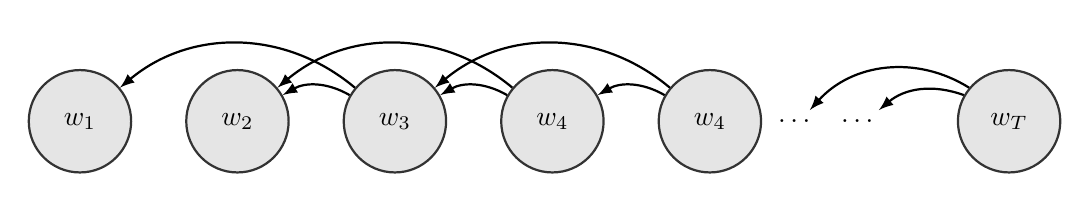
\begin{tikzpicture}
\tikzstyle{main}=[circle, minimum size = 13mm, thick, draw =black!80, node distance = 20mm]
\tikzstyle{obsv}=[main, fill = black!10]
\tikzstyle{hidden}=[node distance = 16mm]
\tikzstyle{connect}=[-latex, thick]
\tikzstyle{box}=[rectangle, draw=black!100]

  \node[obsv] (w1)                {$w_1$};
  \node[obsv] (w2) [right of =w1] {$w_2$};
  \node[obsv] (w3) [right of =w2] {$w_3$};
  \node[obsv] (w4) [right of =w3] {$w_4$};
  \node[obsv] (w5) [right of =w4] {$w_4$};
  \node[hidden] (wI1) [right of =w5, xshift=-5mm] {$\dots$};
  \node[hidden] (wI2) [right of =wI1, xshift=-8mm] {$\dots$};
  \node[obsv] (wT) [right of=wI2, xshift=-1mm] {$w_T$};

  \path (w3) edge [connect, bend right=40] (w1)
        (w3) edge [connect, bend right=30] (w2)
        (w4) edge [connect, bend right=40] (w2)
        (w4) edge [connect, bend right=30] (w3)
        (w5) edge [connect, bend right=40] (w3)
        (w5) edge [connect, bend right=30] (w4)
        (wT) edge [connect, bend right=40] (wI1)
        (wT) edge [connect, bend right=30] (wI2);

\end{tikzpicture}
\caption{Trigram model showing conditional dependencies}
\end{figure} 

\begin{figure}
\centering
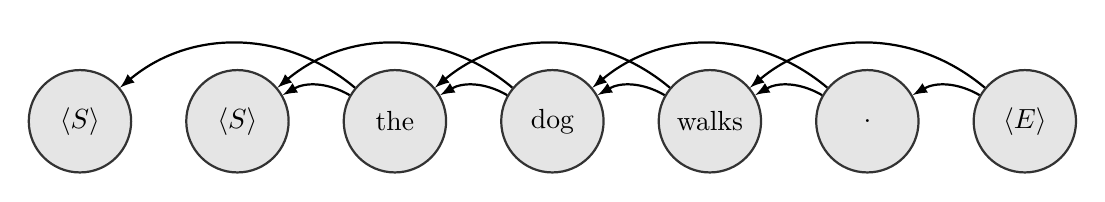
\begin{tikzpicture}
\tikzstyle{main}=[circle, minimum size = 13mm, thick, draw =black!80, node distance = 20mm]
\tikzstyle{obsv}=[main, fill = black!10]
\tikzstyle{hidden}=[node distance = 16mm]
\tikzstyle{connect}=[-latex, thick]
\tikzstyle{box}=[rectangle, draw=black!100]

  \node[obsv] (w1)                {\ngramstart};
  \node[obsv] (w2) [right of =w1] {\ngramstart};
  \node[obsv] (w3) [right of =w2] {the};
  \node[obsv] (w4) [right of =w3] {dog};
  \node[obsv] (w5) [right of =w4] {walks};
  \node[obsv] (w6) [right of =w5] {.};
  \node[obsv] (w7) [right of =w6] {\ngramend};

  \path (w3) edge [connect, bend right=40] (w1)
        (w3) edge [connect, bend right=30] (w2)
        (w4) edge [connect, bend right=40] (w2)
        (w4) edge [connect, bend right=30] (w3)
        (w5) edge [connect, bend right=40] (w3)
        (w5) edge [connect, bend right=30] (w4)
        (w6) edge [connect, bend right=40] (w4)
        (w6) edge [connect, bend right=30] (w5)
        (w7) edge [connect, bend right=40] (w5)
        (w7) edge [connect, bend right=30] (w6);

\end{tikzpicture}
\caption{Trigram Model for the sentence ``the dog walks .''}
\end{figure} 





\section{N-Gram Model of Sentences}

\begin{itemize}
  \item Sentences are sequences of words, but with starts and ends.
  \item We also want to model the likelihood of words being at the beginning/end of a sentence.
  \item Append special ``words'' to the sentence
    \begin{itemize}
      \item $n$--1 `\ngramstart' symbols to beginning 
      \item only one `\ngramend' to then end needed
        \begin{itemize}
          \item $p(\ngramend\ \mid\ .\ \ngramend) = 1.0$ since \ngramend\ would always be followed by \ngramend.
        \end{itemize}
    \end{itemize}
  \item ``the man walks the dog .'' (trigrams)
    \begin{itemize}
      \item Becomes ``\ngramstart\ \ngramstart\ the man walks the dog . \ngramend''
      \item $p(\text{\ngramstart\ \ngramstart\ the man walks the dog . \ngramend}) = \\
      ~~~~~~ p(\text{the} \mid \text{\ngramstart\ \ngramstart}) \\
      ~~~~~~ \cdot p(\text{man} \mid \text{\ngramstart\ the}) \\
      ~~~~~~ \cdot p(\text{walks} \mid \text{the man}) \\
      ~~~~~~ \cdot p(\text{the} \mid \text{man walks}) \\
      ~~~~~~ \cdot p(\text{dog} \mid \text{walks the}) \\
      ~~~~~~ \cdot p(\text{.} \mid \text{the dog}) \\
      ~~~~~~ \cdot p(\ngramend \mid \text{dog .})$
    \end{itemize}
  \item Can be generalized to model longer texts: paragraphs, documents, etc:
    \begin{itemize}
      \item Good: can model ngrams that cross sentences (e.g. $p(w_0 \mid .)$ or $p(w_0 \mid\ ?)$)
      \item Bad: more sparsity on \ngramstart\ and \ngramend\
    \end{itemize}  
\end{itemize}


\section{Sentence Likelihood Examples}

Example dataset:
\vspace{-2mm}
\begin{verbatim}
    <S> the dog runs . <E>
    <S> the dog walks . <E>
    <S> the man walks . <E>
    <S> a man walks the dog . <E>
    <S> the cat walks . <E>
    <S> the dog chases the cat . <E>
\end{verbatim}

Sentence Likelihood with Bigrams:

~~~~ $p(\ngramstart\ \text{the dog walks . \ngramend}) \vspace{2mm} \\
~~~~~~~~~~ =  p(\text{the} \mid \ngramstart) \cdot 
              p(\text{dog} \mid \text{the}) \cdot 
              p(\text{walks} \mid \text{dog}) \cdot
              p(\text{.} \mid \text{walks}) \cdot
              p(\text{\ngramend} \mid \text{.}) \vspace{2mm} \\
~~~~~~~~~~ =  \frac{C(\text{\ngramstart\ the})}{\sum_{x \in V-\ngramend} C(\text{\ngramstart\ } x)} \cdot 
              \frac{C(\text{the dog})}{\sum_{x \in V} C(\text{the } x)} \cdot 
              \frac{C(\text{dog walks})}{\sum_{x \in V} C(\text{dog } x)} \cdot
              \frac{C(\text{walks .})}{\sum_{x \in V} C(\text{walks } x)} \cdot
              \frac{C(\text{. \ngramend})}{\sum_{x \in V} C(\text{. } x)} \vspace{2mm} \\
~~~~~~~~~~ =  \frac{C(\text{\ngramstart\ the})}{C(\text{\ngramstart})} \cdot 
              \frac{C(\text{the dog})}{C(\text{the})} \cdot 
              \frac{C(\text{dog walks})}{C(\text{dog})} \cdot
              \frac{C(\text{walks .})}{C(\text{walks})} \cdot
              \frac{C(\text{. \ngramend})}{C(\text{.})} \vspace{2mm} \\
~~~~~~~~~~ =  \frac{5}{6} \cdot 
              \frac{4}{7} \cdot 
              \frac{1}{4} \cdot
              \frac{3}{4} \cdot
              \frac{6}{6} = 
              0.83 \cdot 0.57 \cdot 0.25 \cdot 0.75 \cdot 1.0 = \mathbf{0.089} $
\\\\

~~~~ $p(\ngramstart\ \text{the cat walks the dog . \ngramend}) \vspace{2mm} \\
~~~~~~~~~~ =  p(\text{the} \mid \ngramstart) \cdot 
              p(\text{cat} \mid \text{the}) \cdot 
              p(\text{walks} \mid \text{cat}) \cdot
              p(\text{the} \mid \text{walks}) \cdot
              p(\text{dog} \mid \text{the}) \cdot
              p(\text{.} \mid \text{dog}) \cdot
              p(\text{\ngramend} \mid \text{.}) \vspace{2mm} \\
~~~~~~~~~~ =  \frac{C(\text{\ngramstart\ the})}{\sum_{x \in V-\ngramend} C(\text{\ngramstart\ } x)} \cdot 
              \frac{C(\text{the cat})}{\sum_{x \in V} C(\text{the } x)} \cdot 
              \frac{C(\text{cat walks})}{\sum_{x \in V} C(\text{cat } x)} \cdot
              \frac{C(\text{walks the})}{\sum_{x \in V} C(\text{walks } x)} \cdot
              \frac{C(\text{the dog})}{\sum_{x \in V} C(\text{the } x)} \cdot
              \frac{C(\text{dog .})}{\sum_{x \in V} C(\text{dog } x)} \cdot
              \frac{C(\text{. \ngramend})}{\sum_{x \in V} C(\text{. } x)} \vspace{2mm} \\
~~~~~~~~~~ =  \frac{C(\text{\ngramstart\ the})}{C(\text{\ngramstart})} \cdot 
              \frac{C(\text{the cat})}{C(\text{the})} \cdot 
              \frac{C(\text{cat walks})}{C(\text{cat})} \cdot
              \frac{C(\text{walks the})}{C(\text{walks})} \cdot
              \frac{C(\text{the dog})}{C(\text{the})} \cdot
              \frac{C(\text{dog .})}{C(\text{dog})} \cdot
              \frac{C(\text{. \ngramend})}{C(\text{.})} \vspace{2mm} \\
~~~~~~~~~~ =  \frac{5}{6} \cdot 
              \frac{1}{7} \cdot 
              \frac{1}{1} \cdot
              \frac{1}{4} \cdot
              \frac{4}{7} \cdot 
              \frac{1}{4} \cdot
              \frac{6}{6} = 
              0.83 \cdot 0.14 \cdot 1.0 \cdot 0.25 \cdot 0.57 \cdot 0.25 \cdot 1.0 = \mathbf{0.004} $
\\\\

~~~~ $p(\ngramstart\ \text{the cat runs . \ngramend}) \vspace{2mm} \\
~~~~~~~~~~ =  p(\text{the} \mid \ngramstart) \cdot 
              p(\text{cat} \mid \text{the}) \cdot 
              p(\text{runs} \mid \text{cat}) \cdot
              p(\text{.} \mid \text{runs}) \cdot
              p(\text{\ngramend} \mid \text{.}) \vspace{2mm} \\
~~~~~~~~~~ =  \frac{C(\text{\ngramstart\ the})}{\sum_{x \in V} C(\text{\ngramstart\ } x)} \cdot 
              \frac{C(\text{the cat})}{\sum_{x \in V} C(\text{the } x)} \cdot 
              \frac{C(\text{cat runs})}{\sum_{x \in V} C(\text{cat } x)} \cdot
              \frac{C(\text{runs .})}{\sum_{x \in V} C(\text{runs } x)} \cdot
              \frac{C(\text{. \ngramend})}{\sum_{x \in V} C(\text{. } x)} \vspace{2mm} \\
~~~~~~~~~~ =  \frac{C(\text{\ngramstart\ the})}{C(\text{\ngramstart})} \cdot 
              \frac{C(\text{the cat})}{C(\text{the})} \cdot 
              \frac{C(\text{cat runs})}{C(\text{cat})} \cdot
              \frac{C(\text{runs .})}{C(\text{runs})} \cdot
              \frac{C(\text{. \ngramend})}{C(\text{.})} \vspace{2mm} \\
~~~~~~~~~~ =  \frac{5}{6} \cdot 
              \frac{1}{7} \cdot 
              \frac{\mathbf{0}}{1} \cdot
              \frac{1}{1} \cdot
              \frac{6}{6} = 
              0.83 \cdot 0.14 \cdot \mathbf{0.0} \cdot 1.0 \cdot 1.0 = \mathbf{0.000} $

\begin{itemize}
  \item Longer sentences have lower likelihoods.
    \begin{itemize}
      \item This makes sense because longer sequences are harder to match exactly.
    \end{itemize}
  \item Zeros happen when an n-gram isn't seen.
\end{itemize}



~\\ \bs\bs~ Day 3

\section{Handling Sparsity}

How big of a problem is sparsity?

\begin{itemize}
  \item Alice's Adventures in Wonderland
    \begin{itemize}
      \item Vocabulary (all word types) size: $V=$ 3,569
      \item Distinct bigrams:  17,149; $\frac{17,149}{|V|^2}$, or 99.8\% of possible bigrams unseen
      \item Distinct trigrams: 28,540; $\frac{17,149}{|V|^3}$, or 99.9999994\% of possible trigrams unseen
    \end{itemize}
  \item If a sequence contains an unseen ngram, it will have likelihood zero: an impossible sequence.
  \item Many legitimate ngrams will simply be absent from the corpus.
  \item This does not mean they are impossible.
  \item Even ungrammatical/nonsense ngrams should not cause an entire sequence's likelihood to be zero.
  \item Many others will be too infrequent to estimate well.
\end{itemize}


Add-$\lambda$ Smoothing

\begin{itemize}
  \item Add some constant $\lambda$ to every count, including unseen ngrams
  \item $V$ is the Vocabulary --- all posslb ``next word'' types --- including \ngramend\ (if necessary $n>1$)
    \begin{itemize}
      \item Don't need \ngramstart\ because it will never be the `next word'
    \end{itemize}
  \item $p(w_0 \mid w_{1-n}~...~w_{-1}) = 
         \frac{C(w_{1-n}~...~w_{-1}~w_0)+\lambda}{\sum_{x \in V} (C(w_{1-n}~...~w_{-1}~x) + \lambda)} =
         \frac{C(w_{1-n}~...~w_{-1}~w_0)+\lambda}{(\sum_{x \in V} C(w_{1-n}~...~w_{-1}~x))+\lambda|V|} =
         \frac{C(w_{1-n}~...~w_{-1}~w_0)+\lambda}{C(w_{1-n}~...~w_{-1})+\lambda|V|}$
  \begin{itemize}
    \item Add $|V|$ to denominator to account for the fact that there is an extra count for every $x$
  \end{itemize}
  \item In practice it over-smoothes, even when $\lambda < 1$
  \item 
Example dataset:
\vspace{-2mm}
\begin{verbatim}
    <S> <S> the dog runs . <E>
    <S> <S> the dog walks . <E>
    <S> <S> the man walks . <E>
    <S> <S> a man walks the dog . <E>
    <S> <S> the cat walks . <E>
    <S> <S> the dog chases the cat . <E>
\end{verbatim}

$V = \{a, cat, chases, dog, man, runs, the, walks, ., \ngramend \}$\\
$|V| = 10$

Sentence Likelihood with Trigrams:

~~~~ $p(\text{``the cat runs .''}) \vspace{2mm} \\
~~~~~~~~ =  p(\ngramstart\ \ngramstart\ \text{the cat runs . \ngramend}) \vspace{2mm} \\
~~~~~~~~ =  p(\text{the} \mid \ngramstart~\ngramstart) \cdot 
              p(\text{cat} \mid \ngramstart \text{ the}) \cdot 
              p(\text{runs} \mid \text{the cat}) \cdot
              p(\text{.} \mid \text{cat runs}) \cdot
              p(\text{\ngramend} \mid \text{runs .}) \vspace{2mm} \\
~~~~~~~~ =    \frac{C(\text{\ngramstart\ \ngramstart\ the})}{\sum_{x \in V} (C(\text{\ngramstart\ \ngramstart\ } x)+1)} \cdot 
              \frac{C(\text{\ngramstart\ the cat})+1}{\sum_{x \in V} (C(\text{\ngramstart\ the } x)+1)} \cdot 
              \frac{C(\text{the cat runs})+1}{\sum_{x \in V} (C(\text{the cat } x)+1)} \cdot
              \frac{C(\text{cat runs .})+1}{\sum_{x \in V} (C(\text{cat runs } x)+1)} \cdot
              \frac{C(\text{runs . \ngramend})+1}{\sum_{x \in V} (C(\text{runs . } x)+1)} \vspace{2mm} \\
~~~~~~~~ =    \frac{C(\text{\ngramstart\ \ngramstart\ the})+1}{C(\text{\ngramstart\ \ngramstart})+(|V|-1)} \cdot 
              \frac{C(\text{\ngramstart\ the cat})+1}{C(\text{\ngramstart\ the})+|V|} \cdot 
              \frac{C(\text{the cat runs})+1}{C(\text{the cat})+|V|} \cdot
              \frac{C(\text{cat runs .})+1}{C(\text{cat runs})+|V|} \cdot
              \frac{C(\text{runs . \ngramend})+1}{C(\text{runs .})+|V|} \vspace{2mm} \\
~~~~~~~~ =    \frac{5+1}{6+\mathbf{9}} \cdot 
              \frac{1+1}{5+10} \cdot 
              \frac{\mathbf{0}+1}{\mathbf{2}+10} \cdot
              \frac{\mathbf{0}+1}{\mathbf{0}+10} \cdot
              \frac{1+1}{1+10} \vspace{2mm} \\
~~~~~~~~ =    0.40 \cdot 0.13 \cdot \mathbf{0.08} \cdot \mathbf{0.10} \cdot 0.18 = \mathbf{0.000081} $

  \item If the context was never seen, then the distribution is uniform: 
    \begin{align*}
      p_{+\lambda}(w_0 \mid w_{-2}, w_{-1}) &= \frac{C(w_{-2}~w_{-1}~w_{0})+\lambda}{\left(\sum_{x \in V} C(w_{-2}~w_{-1}~x)\right)+ \lambda \cdot |V|} \\
                                 &= \frac{0+\lambda}{\left(\sum_{x \in V} 0\right) + \lambda \cdot |V|} \\
                                 &= \frac{0+\lambda}{0+\lambda \cdot |V|}
                                 = \frac{\lambda}{\lambda \cdot |V|}
                                 = \frac{1}{1 \cdot |V|}
                                 = \frac{1}{|V|}
    \end{align*}
  \item Since \ngramstart\ can never be followed by \ngramend
    \begin{itemize}
      \item $p(\ngramend \mid \ngramstart~\ngramstart) = 0$
      \item The denominator $\sum_{x \in V} C(\ngramstart~\ngramstart~x)$ only gets $|V|$-1 smoothing counts
    \end{itemize}
  \item \ngramstart\ not included in $V$ because we can't transition to it.

  \item More smoothing on less common ngrams
    \begin{itemize}
      \item With smoothing, we have counts for any possible type following ``runs .'': \vspace{1mm} \\
      ~~~~~~~~ $p(\ngramend \mid$ runs .$) = \frac{1+1}{1 + 10} = \frac{2}{11} = 0.18$ \vspace{1mm} \\
      ~~~~~~~~ $p($the $\mid$ runs .$) = \frac{0+1}{1 + 10} = \frac{1}{11} = 0.09$ \vspace{1mm} 
      \begin{itemize}
        \item Counts of ``runs .'' are very low (only 1 occurrence), so estimates are bad
        \item Bad estimates means more smoothing is good
        \item MLE of ``runs . \ngramend'' is 1.0, add-1 smoothed becomes 0.18 \vspace{1mm} \\
              MLE of ``runs . the'' is 0.0, add-1 smoothed becomes 0.09
        \item Original difference of 1.0 becomes difference of 0.09!
        \item This makes sense because our estimates are so bad that we really can't make a judgement about what could possibly follow ``runs .''
      \end{itemize}
      \item Contexts with higher counts have less smoothing: \vspace{1mm} \\
      ~~~~~~~~ $p(\ngramend \mid$ walks .$) = \frac{3+1}{3 + 10} = \frac{4}{13} = 0.31$ \vspace{1mm} \\
      ~~~~~~~~ $p($the $\mid$ walks .$) = \frac{0+1}{3 + 10} = \frac{1}{13} = 0.08$ \vspace{1mm} 
      \begin{itemize}
        \item Counts of ``walks .'' are higher (3 occurrence), so estimates are better
        \item Better estimates means less smoothing is good
        \item MLE of ``walks . \ngramend'' is 1.0, add-1 smoothed becomes 0.31 \vspace{1mm} \\
              MLE of ``walks . the'' is 0.0, add-1 smoothed becomes 0.08
        \item Original difference of 1.0 becomes difference of 0.23
        \item Remains a larger gap than we saw for ``runs . $x$''
        \item This makes sense because our estimates are better, so we can be more sure that ``walks .'' should only be followed by \ngramend
      \end{itemize}
    \end{itemize}

  \item Disadvantages of add-$\lambda$ smoothing:
    \begin{itemize}
      \item Over-smoothes.
    \end{itemize}


\end{itemize}

Good-Turing Smoothing

\begin{itemize}
  \item Estimate counts of things you haven't seen from counts of things you have
  \item Estimate probability of things which occur $c$ times with the probability of things which occur $c+1$ times
  \item $c^* = (c+1) \frac{N_{c+1}}{N_c}$ \vspace{2mm} \\
        $p^*_{GT}(\textit{things with freq 0}) = \frac{N_1}{N}$
  \item $p_{GT}(w_0 \mid w_{1-n}~...~w_{-1}) = 
         \frac{C^*(w_{1-n}~...~w_{-1}~w_0)}{C^*(w_{1-n}~...~w_{-1})}$
\end{itemize}


Knesser-Ney Smoothing

\begin{itemize}
  \item Intuition: interpolate based on ``openness'' of the context
  \item Words seen in more contexts are more likely to appear in others
  \item Even if we haven't seen $w_0$ following the context, if the context is ``open'' (supports a wide variety of ``next words''), then it is more likely to support $w_0$
  \item Boost counts based on $|\{x : C(w_{1-n}~...~w_{-1}~x)>0\}|$, the number of different ``next words'' seen after $w_{1-n}~...~w_{-1}$
\end{itemize}



~\\ \bs\bs~ Day 4 \\

Interpolation

\begin{itemize}
  \item Mix n-gram probability with probabilities from lower-order models
    \begin{align*}
      \hat{p}(w_0 \mid w_{-2}~w_{-1}) &= ~~~~ \lambda_3 \cdot p(w_0 \mid w_{-2}~w_{-1}) &&&& \\
                                        &~~~~+ \lambda_2 \cdot p(w_0 \mid w_{-1}) \\
                                        &~~~~+ \lambda_1 \cdot p(w_0)
    \end{align*}
  \item $\lambda_i$ terms used to decide how much to smooth
  \item $\sum_i \lambda_i = 1$ (still a valid probability distribution, because they are proportions
  \item Use \textit{dev} dataset to tune $\lambda$ hyperparameters
  \item Also useful for combining models trained on different data:
  \begin{itemize}
    \item Can interpolate ``customized'' models with ``general'' models
    \item Baseline English + regional English + user-specific English
    \item Little in-domain data, lots of out-of-domain
  \end{itemize}
\end{itemize}


Stupid Backoff

\begin{itemize}
  \item If p(n-gram)=0, just use p((n-1)-gram)
  \item Does \textit{not} yield a valid probability distribution
  \item Works shockingly well for huge datasets
\end{itemize}


\section{Out-of-Vocabulary Words (OOV)}

Add-$\lambda$

\begin{itemize}
  \item If ngram contains OOV item, assume count of $\lambda$, just like for all other ngrams.
  \item Probability distributions become invalid.  We can't know the full vocabulary size, so we can't normalize counts correctly.
\end{itemize}


\ngramunk

\begin{itemize}
  \item Create special token \ngramunk
  \item Create a fixed lexicon $L$
    \begin{itemize}
      \item All types in some subset of training data?
      \item All types appearing more than $k$ times?
    \end{itemize}
  \item $V = L + \ngramunk$, ~ $|V| = |L|+1$
  \item Before training, change any word not in $L$ to \ngramunk
  \item Then train as usual as if \ngramunk was a normal word
  \item For new sentence, again replace words not in $L$ with \ngramunk before using model
  \item Probabilities containing \ngramunk\ measure likelihood with \textit{some rare word}
  \item Problem: the ``rare'' word is no longer rare since there are many \ngramunk tokens
    \begin{itemize}
      \item Ngrams with \ngramunk will have higher probabilities than those with any particular rare word
      \item Not so bad when comparing same sequence under multiple models.  All will have inflated probabilities.
      \item More problematic when comparing probabilities of different sequences under the same model
        \begin{itemize}
          \item p(i \textbf{totes} know) $<$ p(i \textbf{totally} know) $<$ p(i $\mathbf{\langle unk \rangle}$\ know)
        \end{itemize}
    \end{itemize}
\end{itemize}




\section{Evaluation}

Extrinsic

\begin{itemize}
  \item Use the model in some larger task.  See if it helps.
  \item More realistic
  \item Harder
\end{itemize}

Intrinsic

\begin{itemize}
  \item Evaluate on a test corpus
  \item Easier
\end{itemize}

Perplexity

\begin{itemize}
  \item Intrinsic measure of model quality
  \item How well does the model ``fit'' the test data?
  \item How ``perplexed'' is the model whe it sees the test data?
  \item Measure the probability of the test corpus, normalize for number of words.
  \item $PP(W) = \sqrt[|W|]{\frac{1}{p(w_1~w_2~...~w_{|W|})}}$
  \item With individual sentences: $PP(s_1, s_2, ...) = \sqrt[(\sum_i |s_i|)]{\frac{1}{\prod_i p(s_i)}}$
\end{itemize}






\section{Generative Models}

\begin{itemize}
  \item Generative models are designed to model how the data \textit{could have been generated}.
  \item The best parameters are those that would most likely generate the data.
  \item MLE maximizes that likelihood that the training data was generated by the model.
  \item As such, we can \textit{actually generate} data from a model.
 
  \item Trigram model:
    \begin{itemize}
      \item General:
        \begin{itemize}
          \item[] \hspace{-4mm} For each sequence:
            \begin{enumerate}
              \item Sample a word $w_0$ according to $w_0 \sim p(w_0)$
              \item Sample a second word $w_1$ according to $w_1 \sim p(w_1 \mid w_0)$
              \item Sample a next word $w_k$ according to $w_k \sim p(w_k \mid w_{k-2}~w_{k-1})$
              \item Repeat step 3 until you feel like stopping.
            \end{enumerate}
        \end{itemize}
      \item Sentences:
        \begin{itemize}
          \item[] \hspace{-4mm} For each sentence:
            \begin{enumerate}
              \item Sample a word $w_0$ according to $w_0 \sim p(w_0 \mid \ngramstart~\ngramstart)$
              \item Sample a second word $w_1$ according to $w_1 \sim p(w_1 \mid w_0~\ngramstart)$
              \item Sample a next word $w_k$ according to $w_k \sim p(w_k \mid w_{k-2}~w_{k-1})$
              \item Repeat until $\ngramend$ is drawn.
            \end{enumerate}
        \end{itemize}
    \end{itemize}

  \item Longer $n$ generates more coherent text
  \item Too-large $n$ just ends up generating sentences from the training data because most counts will be 1 (no choice of next word).

  \item Na\"{i}ve Bayes was a generative model too!
    \begin{itemize}
      \item[] \hspace{-4mm} For each instance:
        \begin{enumerate}
          \item Sample a label $l$ according to $l \sim p(Label=l)$          
          \item For each feature $F$: sample a value $v$ according to $v \sim p(F=v \mid Label=l)$
        \end{enumerate}
    \end{itemize}

  \item We will see many more generative models throughout this course
\end{itemize}


\begin{figure}
\centering
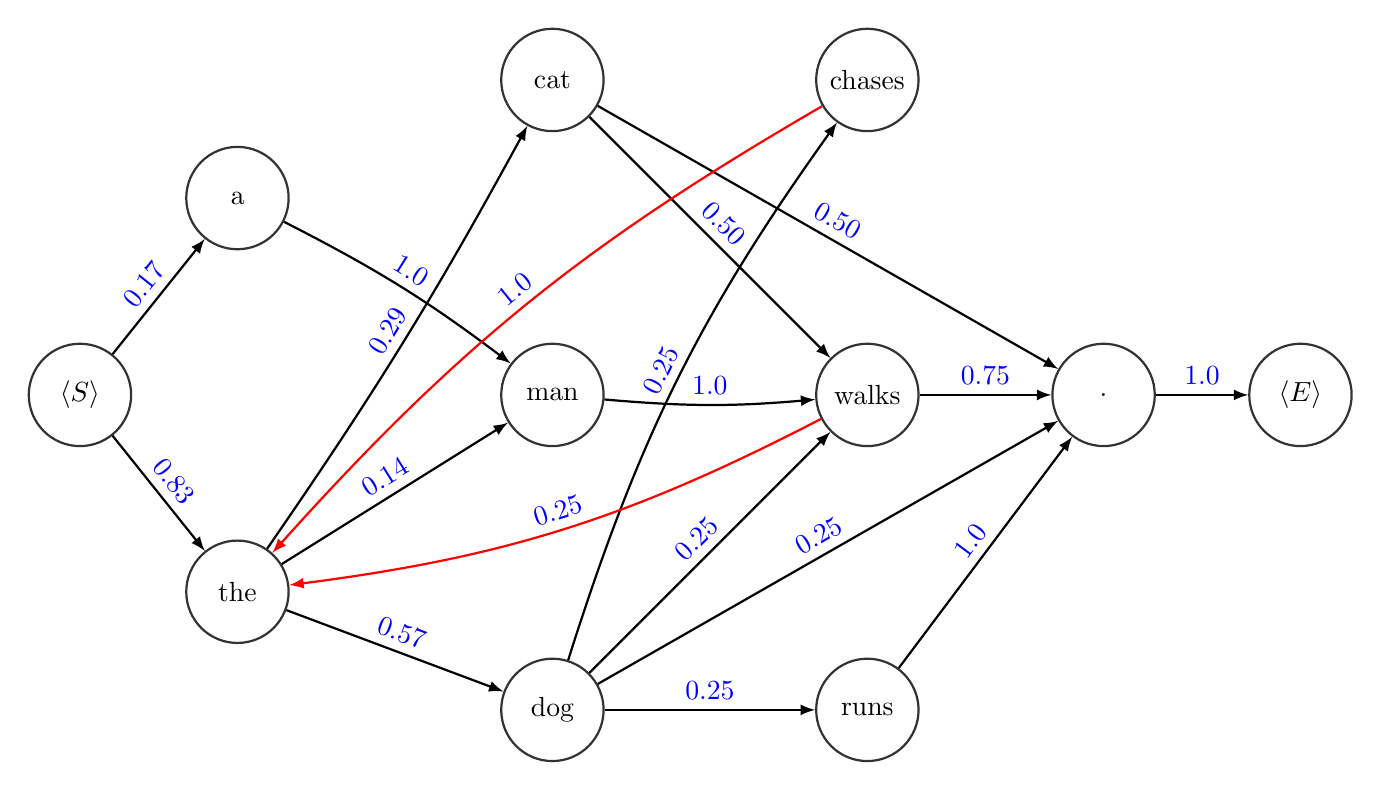
\begin{tikzpicture}
\tikzstyle{main}=[circle, minimum size = 13mm, thick, draw =black!80, node distance = 40mm]
\tikzstyle{obsv}=[main, fill = black!10]
\tikzstyle{hidden}=[node distance = 16mm]
\tikzstyle{connect}=[-latex, thick]
\tikzstyle{box}=[rectangle, draw=black!100]

  \node[main] (start)                {\ngramstart};

  \node[main] (the)    [right of =start, xshift=-20mm, yshift=-25mm] {the};
  \node[main] (a)      [right of =start, xshift=-20mm, yshift= 25mm] {a};

  \node[main] (man)    [right of =start, xshift=20mm              ] {man};
  \node[main] (dog)    [above of =man,                yshift=-80mm] {dog};
  \node[main] (cat)    [below of =man,                yshift= 80mm] {cat};

  \node[main] (walks)  [right of =man,                ] {walks};
  \node[main] (runs)   [right of =dog,                ] {runs};
  \node[main] (chases) [right of =cat,                ] {chases};

  \node[main] (stop)      [right of =walks, xshift=-10mm]              {.};

  \node[main] (end)    [right of =stop, xshift=-15mm]              {\ngramend};


  \path (start) edge [connect] node [pos=0.5, above, blue, sloped] {0.17} (a);
  \path (start) edge [connect] node [pos=0.5, above, blue, sloped] {0.83} (the);

  \path (the) edge [connect] node [pos=0.5, above, blue, sloped] {0.14} (man);
  \path (the) edge [connect] node [pos=0.5, above, blue, sloped] {0.57} (dog);
  \path (the) edge [connect, bend right=3] node [pos=0.5, above, blue, sloped] {0.29} (cat);
  \path (a) edge [connect, bend left=5] node [pos=0.5, above, blue, sloped] {1.0} (man);
  %\path (a) edge [connect] node [pos=0.5, above, blue, sloped] {label} (dog);
  %\path (a) edge [connect] node [pos=0.5, above, blue, sloped] {label} (cat);

  \path (man) edge [connect, bend right=5] node [pos=0.5, above, blue, sloped] {1.0} (walks);
  %\path (man) edge [connect] node [pos=0.5, above, blue, sloped] {label} (chases);
  \path (dog) edge [connect] node [pos=0.5, above, blue, sloped] {0.25} (walks);
  \path (dog) edge [connect,  bend left=9] node [pos=0.5, above, blue, sloped] {0.25} (chases);
  \path (dog) edge [connect] node [pos=0.5, above, blue, sloped] {0.25} (runs);
  \path (dog) edge [connect] node [pos=0.5, above, blue, sloped] {0.25} (stop);
  \path (cat) edge [connect] node [pos=0.5, above, blue, sloped] {0.50} (walks);
  \path (cat) edge [connect] node [pos=0.5, above, blue, sloped] {0.50} (stop);

  %\path (chases) edge [connect] node [pos=0.5, above, blue, sloped] {label} (stop);
  \path (chases) edge [connect, red, bend right=9] node [pos=0.5, above, blue, sloped] {1.0} (the);
  %\path (chases) edge [connect, bend right=20] node [pos=0.5, above, blue, sloped] {label} (a);
  \path (walks) edge [connect, red, bend left=10] node [pos=0.5, above, blue, sloped] {0.25} (the);
  \path (walks) edge [connect] node [pos=0.5, above, blue, sloped] {0.75} (stop);
  %\path (walks) edge [connect,  bend left=25] node [pos=0.5, above, blue, sloped] {label} (a);
  \path (runs) edge [connect] node [pos=0.5, above, blue, sloped] {1.0} (stop);
  
  \path (stop) edge [connect] node [pos=0.5, above, blue, sloped] {1.0} (end);

\end{tikzpicture}
\caption{Finite state machine.  Missing arrows are assumed to be zero probabilities.  With smoothing, there would be an arrow in \textit{both directions} between \textit{every} pair of words.}
\end{figure} 

\begin{verbatim}
p(S -> the) = 0.83          p(dog -> chases) = 0.25
p(S -> a) = 0.17            p(dog -> runs) = 0.25
                            p(dog -> .) = 0.25
p(the -> cat) = 0.29        p(dog -> walks) = 0.25
p(the -> dog) = 0.57
p(the -> man) = 0.14        p(chases -> the) = 1.00

p(a -> man) = 1.00          p(runs -> .) = 1.00

p(man -> walks) = 1.00      p(walks -> the) = 0.25
                            p(walks -> .) = 0.75
p(cat -> walks) = 0.50
p(cat -> .) = 0.50          p(. -> <E>) = 1.00
\end{verbatim}


\section{How much data?}

Choosing $n$
\begin{itemize}
  \item Large $n$
    \begin{itemize}
      \item More context for probabilities: \\ $p(\text{phone})$ vs \\
                                               $p(\text{phone} \mid \text{cell})$ vs \\
                                               $p(\text{phone} \mid \text{your cell})$ vs \\
                                               $p(\text{phone} \mid \text{off your cell})$ vs \\
                                               $p(\text{phone} \mid \text{turn off your cell})$
      \item Long-range dependencies
    \end{itemize}
  \item Small $n$
    \begin{itemize}
      \item Better generalization
      \item Better estimates
      \item Long-range dependencies
    \end{itemize}
\end{itemize}

How much training data?
\begin{itemize}
  \item \textit{As much as possible.}
  \item More data means better estimates
  \item Google N-Gram corpus uses 10-grams
  \item[] 
      \begin{figure}[h]
        \centering
        \begin{subfigure}[b]{0.3\textwidth}
                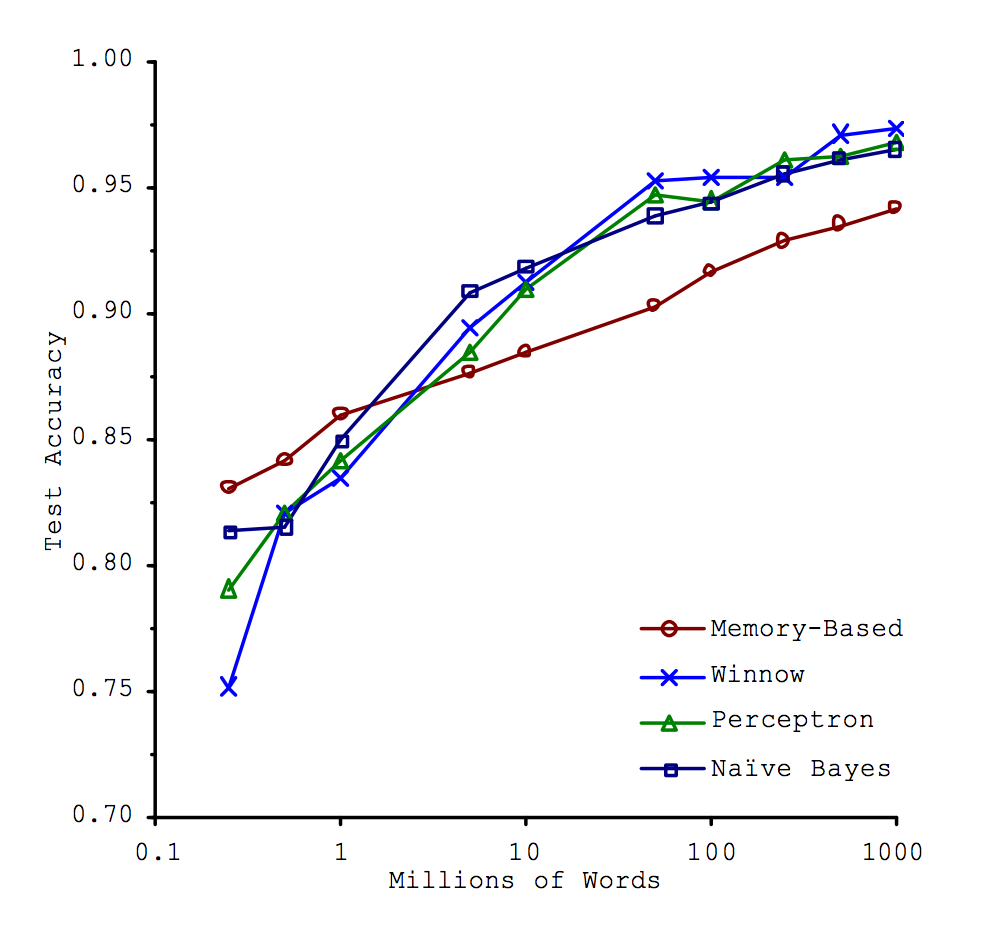
\includegraphics[width=0.95\textwidth]{banko-brill-graph.png}
                \caption{Data size matters more than algorithm (Banko and Brill, 2001)}
        \end{subfigure}%
        ~~~
        \begin{subfigure}[b]{0.3\textwidth}
                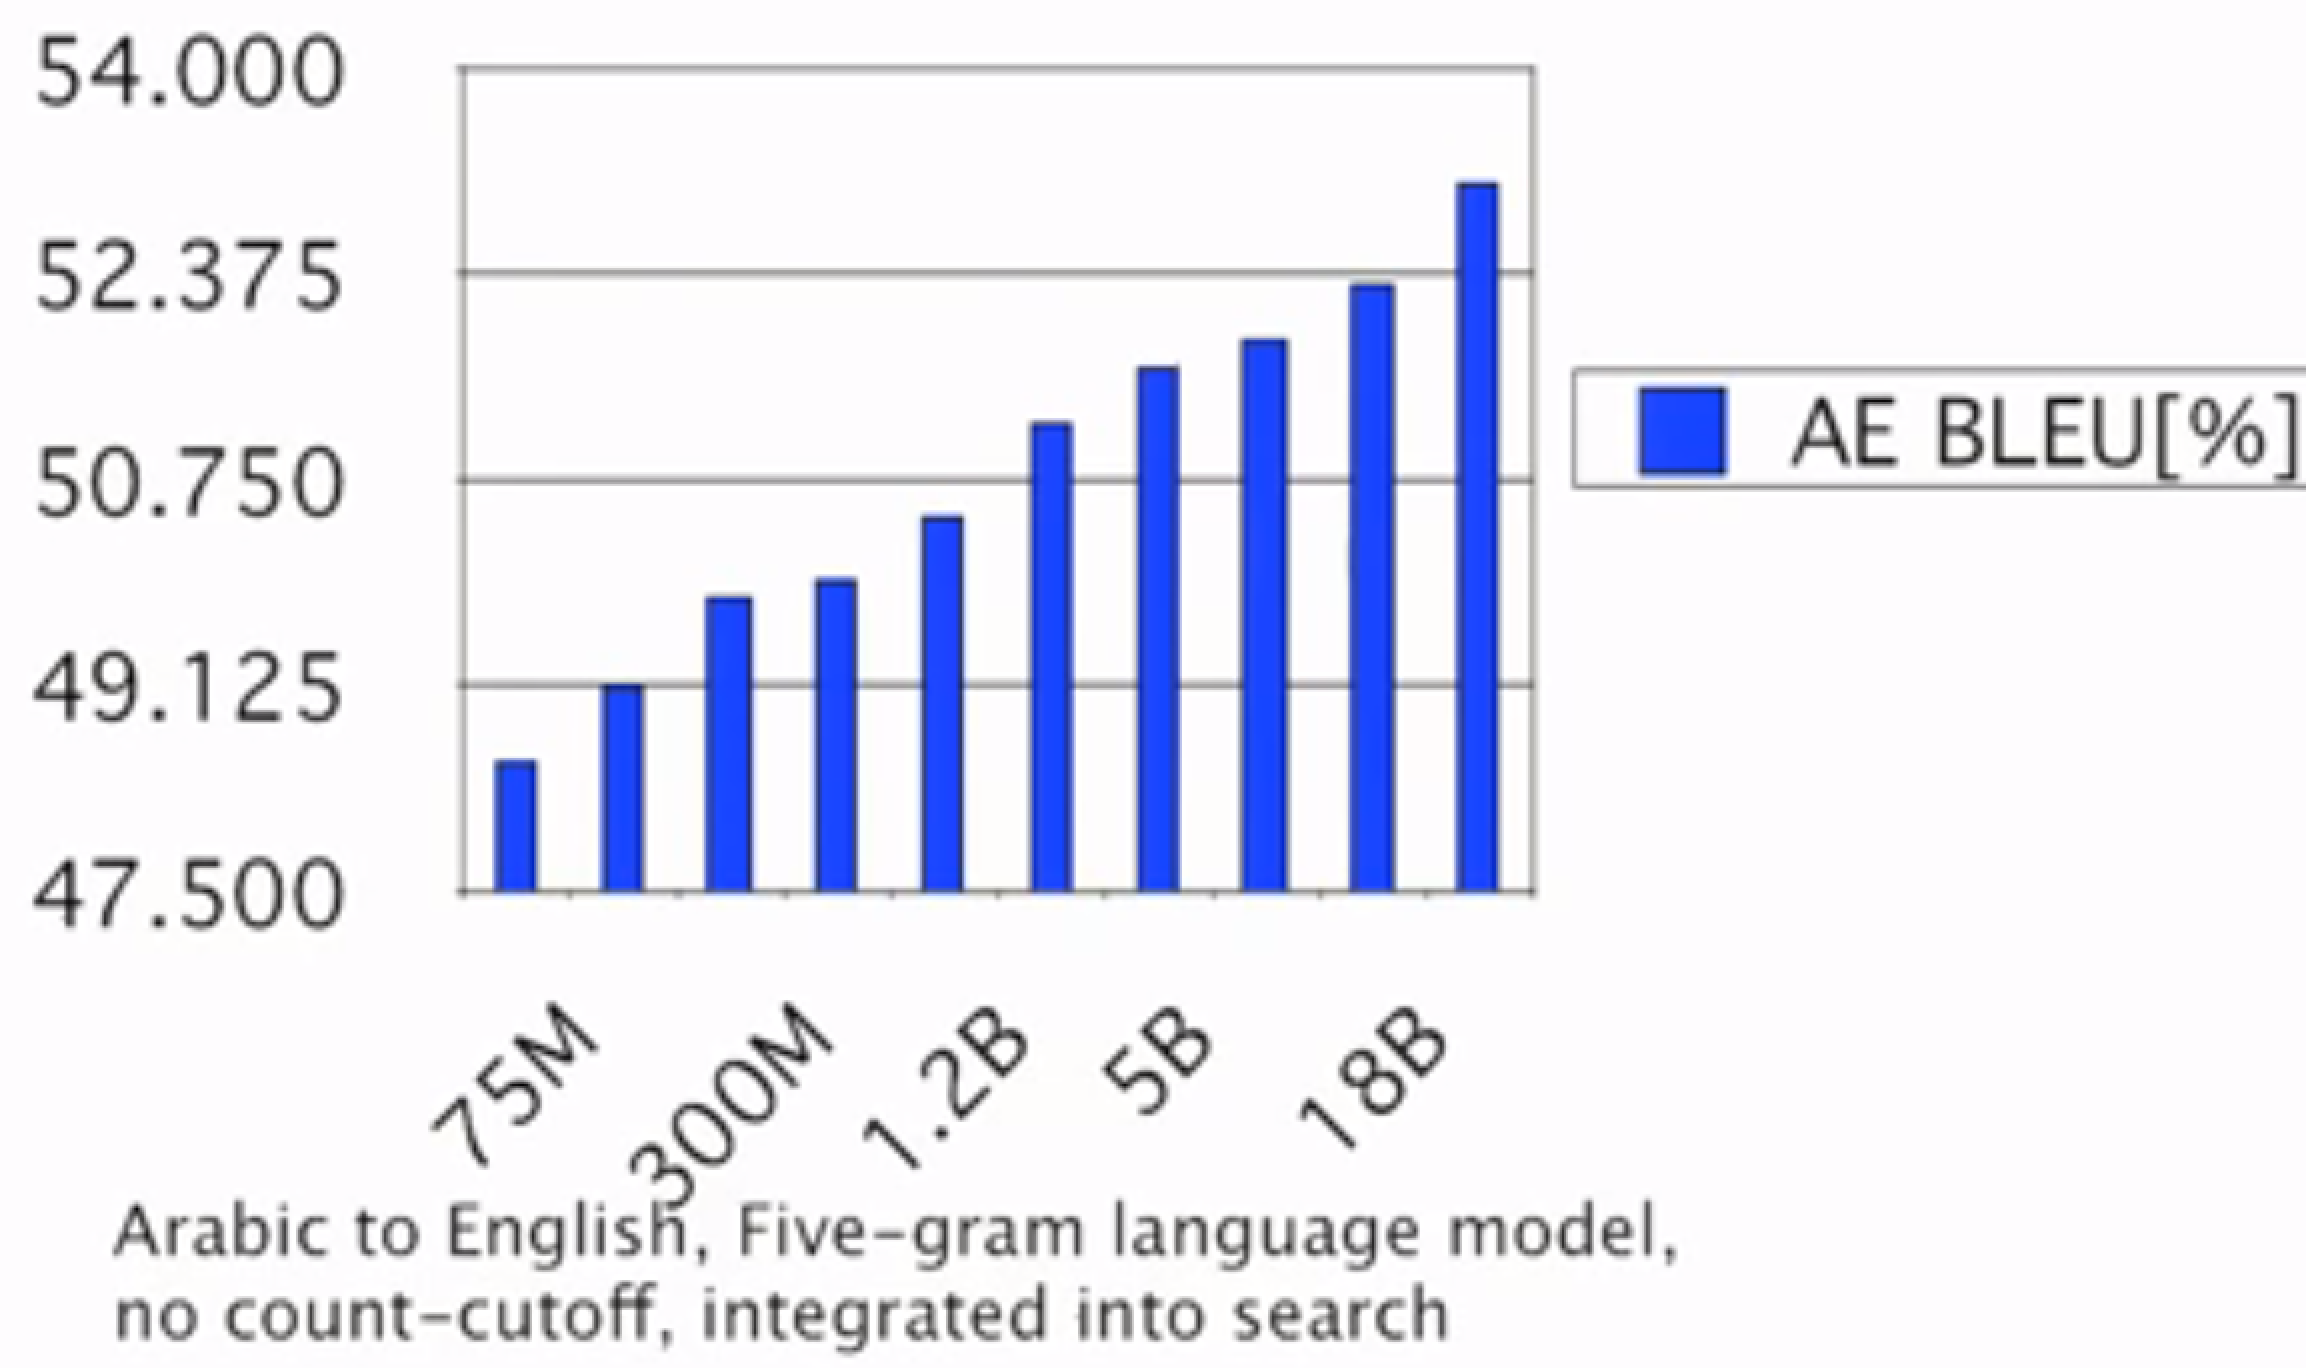
\includegraphics[width=0.95\textwidth]{unreasonable-bleu.png}
                \caption{Results keep improving with more data (Norvig: Unreasonable ...)}
        \end{subfigure}
        ~~~
        \begin{subfigure}[b]{0.3\textwidth}
                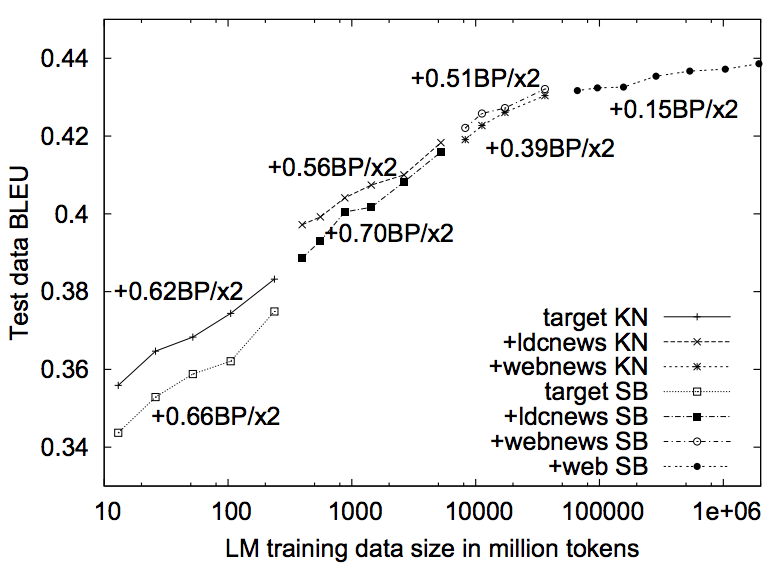
\includegraphics[width=0.95\textwidth]{stupid-backoff.png}
                \caption{With enough data, stupid backoff approaches Knesser-Ney accuracy  (Brants et al., 2007)}
        \end{subfigure}
      \end{figure}
      \vspace{-6mm}
\end{itemize}





\section{Citations}

Some content adapted from:

\begin{itemize}
  \item \url{http://courses.washington.edu/ling570/gina_fall11/slides/ling570_class8_smoothing.pdf}
\end{itemize}


\end{document}

